\documentclass[tikz,border=5pt]{standalone}
\usepackage{fontspec}
\setmainfont{Times New Roman}
\usepackage{unicode-math}
\setmathfont{Cambria Math}
\usetikzlibrary{shapes.geometric,positioning,fit,backgrounds,arrows.meta,calc}

\begin{document}
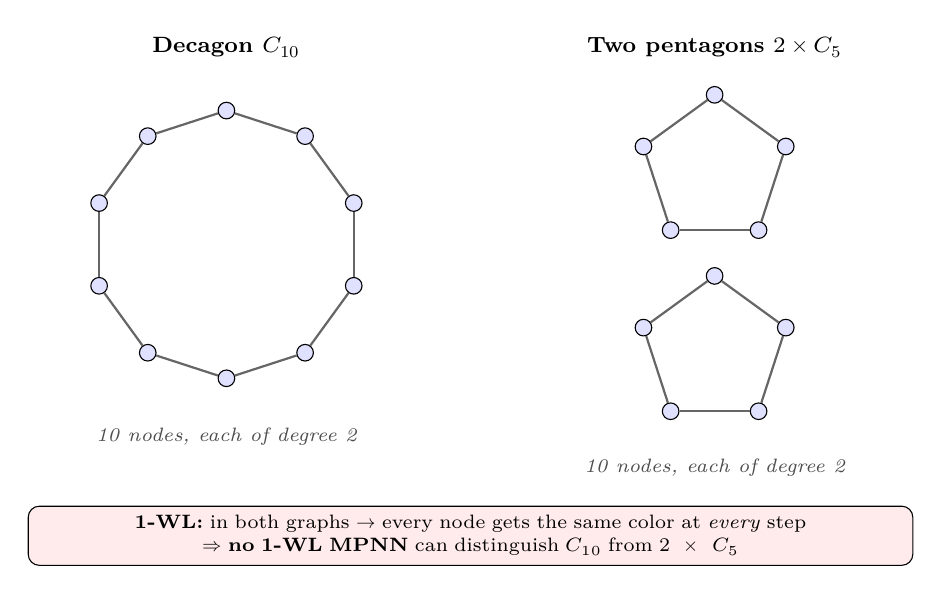
\begin{tikzpicture}[
  nd/.style={circle, draw, fill=blue!12, inner sep=1.6pt, minimum size=6pt},
  label/.style={font=\scriptsize\itshape, text=gray!60!black},
  ttl/.style={font=\footnotesize\bfseries},
]

% ====== Decagon C_10 (left) ======
\node[ttl] at (0, 2.5) {Decagon $C_{10}$};
\foreach \i in {0,...,9} {
  \node[nd] (d\i) at ({90+\i*36}:1.7) {};
}
\foreach \i [evaluate={\j=int(mod(\i+1,10));}] in {0,...,9} {
  \draw[thick, black!60] (d\i) -- (d\j);
}
\node[label, below=0.1cm] at (0, -2.1) {10 nodes, each of degree 2};

% ====== Two pentagons 2 x C_5 (right) ======
\node[ttl] at (6.2, 2.5) {Two pentagons $2\times C_5$};
\foreach \i in {0,...,4} {
  \node[nd] (p\i) at ($(6.2,0.95)+({90+\i*72}:0.95)$) {};
  \node[nd] (q\i) at ($(6.2,-1.35)+({90+\i*72}:0.95)$) {};
}
\foreach \i [evaluate={\j=int(mod(\i+1,5));}] in {0,...,4} {
  \draw[thick, black!60] (p\i) -- (p\j);
  \draw[thick, black!60] (q\i) -- (q\j);
}
\node[label, below=0.05cm] at (6.2, -2.55) {10 nodes, each of degree 2};

% ====== Equivalence verdict ======
\node[draw, rounded corners, fill=red!8, align=center, font=\scriptsize, text width=11cm]
  (verdict) at (3.1, -3.7)
  {\textbf{1-WL:} in both graphs $\to$ every node gets the same color at \emph{every} step\\
   $\Rightarrow$ \textbf{no 1-WL MPNN} can distinguish $C_{10}$ from $2\times C_5$};

\end{tikzpicture}
\end{document}